\documentclass{article}

\usepackage{polski}
\usepackage[UTF8]{inputenc}
\usepackage{graphicx}
\usepackage{float}
\usepackage[margin=1in]{geometry}
\usepackage{graphicx}
\usepackage{amsmath}
\usepackage{mathtools}
\usepackage{amssymb}
\usepackage{multirow}
\usepackage{changepage}
\usepackage[export]{adjustbox}
\usepackage{wrapfig}
\usepackage{makecell}


\begin{document}

\begin{center}
\bgroup
\def\arraystretch{1.5}
\begin{tabular}{|c|c|c|c|c|c|}
	\hline
	EAIiIB & \multicolumn{2}{|c|}{\begin{tabular}{@{}c@{}}  Autor\end{tabular}} & Rok II & Grupa 5 & Zespół 6  \\
	\hline
	\multicolumn{3}{|c|}{\begin{tabular}{c}Temat: \\ Opracowanie danych pomiarowych \end{tabular}} & 
	\multicolumn{3}{|c|}{\begin{tabular}{c}Numer ćwiczenia: \\ 0 \end{tabular}} \\
	\hline
	Data wykonania & Data oddania & Zwrot do poprawki & Data oddania & Data zaliczenia & Ocena \\[6ex]
	\hline
\end{tabular}
\egroup
\end{center} 

%WSTEP
\section{Cel ćwiczenia}
Zapoznanie się z typowymi metodami opracowania danych pomiarowych i szacowania niepewności w pomiarach laboratoryjnych.

\section{Wstęp teoretyczny}
\subsection{Niepewność pomiaru} 
Niepewność pomiaru – parametr, związany z wynikiem pomiaru, charakteryzujący rozrzut wyników, które można w uzasadniony sposób przypisać wartości mierzonej. Charakteryzuje ona rozrzut wartości (szerokość przedziału), wewnątrz którego można z zadowalającym prawdopodobieństwem usytuować wartość wielkości mierzonej. Z definicji niepewności pomiarowej wynika, że nie może być ona wyznaczona doskonale dokładnie.
\subsection{Wahadło matematyczne}
Wahadłem matematycznym nazywamy punktową masę zwieszoną na nieważkiej nici. Podczas ćwiczenia będziemy korzystać z wahadła i kuli zawieszonej na realnych niciach. Wychylając wahadło z położenia równowagi wprowadzamy je w ruch drgający prosty. Okres drgań takiego wahadła jest określony zależnością: $$T =2\pi\sqrt{\frac{l}{g}} $$

\section{Układ pomiarowy}
Zestaw ćwiczeniowy stanowi kulka zawieszona na nici, którą wprowadza się w ruch drgający. Potrzebne przyrządy pomiarowe to przymiar milimetrowy oraz sekundomierz.

%\begin{wrapfigure}{r}{0.5\textwidth}
\begin{figure}[H]
	\begin{center}
	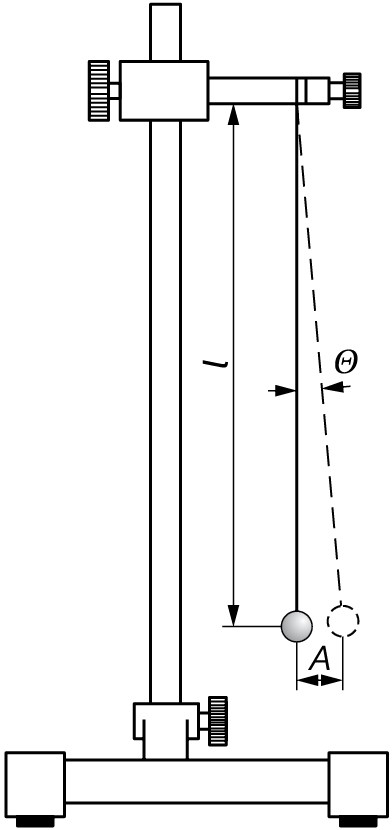
\includegraphics[scale=0.18]{wahadlo.jpg}
	\end{center}
	\caption{Zestaw wahadła prostego}
\end{figure}
%\end{wrapfigure}	
\section{Wykonanie ćwiczenia}
\begin{enumerate}
	\item Pomiar długości wahadła.
	\item Wprowadzenie wahadła w ruch drgający przy wychyleniu nie przekraczającym $10^\circ$. Pomiar 10 okresów drgań.
	\item Powtórzenie pomiarów dla innej długości wahadła.
\end{enumerate}
	

%KONIEC WSTEPU	


\section{Opracowanie wyników}
\begin{enumerate}
	\item Sprawdzenie wyników pomiarów w poszukiwaniu wartości odstających (błędu grubego).
	\item Ustalamy niepewność pomiaru długości wahadła $u(l) = 1$ $[mm]$.
	\item Obliczamy niepewność pomiaru okresu. Dla bardzo małych próbek przyjmujemy $u(T) = 25$ $[ms]$ (czas reakcji człowieka).
	\item Z otrzymanych wyników pomiarów $l$ i $T$, podstawiając do wzoru obliczamy przyspieszenie ziemskie:
	$$g = \frac{4\pi^{2}l}{T^2}$$
	\item Obliczamy niepewność złożoną zmierzonej wartości przyspieszenia ziemskiego $u_{c}(g)$:
	$$ u_{c}(g) = \sqrt{\bigg(\frac{\partial g}{\partial l}u(l)\bigg)^2+\bigg(\frac{\partial g}{\partial T}u(T)\bigg)^2} = \sqrt{\bigg(\frac{4\pi^{2}}{T^{2}}u(l)\bigg)^2+\bigg(-\frac{8\pi^{2}l}{T^{3}}u(T)\bigg)^2} $$
	\item Porównanie uzyskanej wartości przyspieszenia ziemskiego z wartością tabelaryczną $g_{0}=9,811 \frac{m}{s^{2}}$:
	$$ |g-g_{0}|<U(g)=2u_{c}(g)$$
	\item Wyznaczenie prostej regresji i korzystając z niej wyznaczenie przyspieszenia ziemskiego wraz z niepewnością.
\end{enumerate}

\section{Wyniki pomiarów}

\begin{figure}[!htb]
	\begin {table}[H]
	\caption {Podsumowanie wyników} \label{tab} 
	\begin{adjustwidth}{-1cm}{}
		\def\arraystretch{1.3}
		\centering
		\begin{tabular}{|c|c|c|c|c|c|c|c|c|c|}
		
			\hline
			Lp. & $l$ \mbox{[mm]}  & 
			%Liczba zmierzonych okresów & 
			$t$ \mbox{[s]} & $T_{i}$ \mbox{[s]} & $u(T_{i})$ \mbox{[ms]} & $g_{i}$ \mbox{[$\frac{m}{s^2}$]} & $u(g_{i})$ \mbox{[$\frac{m}{s^2}$]} & \makecell{$U(g)$ \mbox{[$\frac{m}{s^2}$]} \\ $k = 2$} & $|g-g_{i}|$  & \makecell{Zgadza się z wartością tabelaryczną \\ $g = 9,811 $  \mbox{[$\frac{m}{s^2}$]}} \\
			\hline
			1 & 398 &
			% 10 & 
			12,63 & 1,264 & 25,07 & 9,838 & 0,3905 & 0,7811 & 0,02809 & Tak
			\\
			\hline
			2 & 485 
			%	& 10
			& 13,85 & 1,385  & 25,95 & 9,986 & 0,3743 & 0,7486 & 0,1749 & Tak
			\\
			\hline
			3 & 161 
			%& 5 
			& 8,066 & 0,8066 & 44,56 & 9,769 & 1,079 & 2,159 & 0,04157 & Tak
			\\
			\hline
			4 & 400 
			%& 5
			& 12,73 & 1,273 & 33,10 & 9,738 & 0,5063 & 1,012 & 0,07254 & Tak
			\\
			\hline
			5 & 281 
			%& 1 
			& 10,60 & 1,060 & 25 & 9,873 & 0,4657 & 0,9314 & 0,06212 & Tak
			\\
			\hline
			6 & 340 
			%	& 1 
			& 11,59 & 1,159 & 25 & 9,992 & 0,4311 & 0,8622 &  0,1814 & Tak
			\\
			\hline
			7 & 540 
			%& 1 
			& 14,72 & 1,472 & 25 & 9.839 & 0,3342 & 0,6684 & 0,02770 & Tak
			\\
			%\hline
		%	Średnia &  
			%& 1 
		%	&  &  &  & 9,862 & 0,3342 & 0,6684 & 0,02770 & Tak
		%	\\
			\hline
		\end{tabular}
	\end{adjustwidth}
\end{table}
\end{figure}
\pagebreak
Po naniesieniu pomiarów wraz z ich niepewnościami można zauważyć, że zależność długości wahadła i okresu nie jest liniowa. Jest to funkcja typu:

$$T = f(l) = k \sqrt{l}$$
gdzie $$ k =  \frac{2 \pi}{\sqrt{g}} $$
\begin{figure}[H]
	\noindent\makebox[\textwidth]{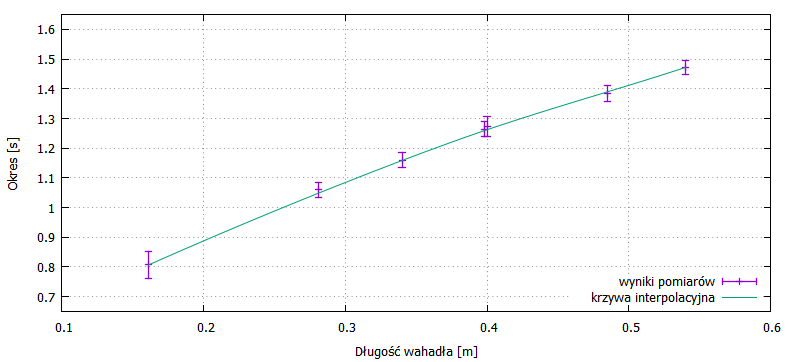
\includegraphics[width=\paperwidth - 50pt]{interpolacja.png}}
	\caption{Wykres zależności okresu od długości wahadła}
\end{figure}

Natomiast zależność długości wahadła i kwadratu okresu jest zbliżona do funkcji liniowej. Obliczyłem więc prostą korzystając z metody najmniejszych kwadratów:
\begin{align*}
&	T^2 = f(l) = 3,984  l \\
&	u(a) = 0,0528 \left[\frac{s^2}{m}\right]
\end{align*}
Porównując oba wzory na $T^2$ otrzymujemy następującą zależność, z której możemy policzyć $g$:
\begin{align*}
& 3,984  l = 4 \pi ^2 \frac{l}{g} \\
& g =  \frac{4 \pi ^2}{ 3,984} = 9,9092 \left[\frac{m}{s^2}\right] \\
& u(g) = \frac{4 \pi ^2 }{a^2}u(a) = 0,131 \left[\frac{m}{s^2}\right] \end{align*}
Sprawdzenie z wartością tabelaryczną:
\begin{align*}
& U(g) = 2u(g) = 0,263 \left[\frac{m}{s^2}\right] \\
&\left|9,811-9,9092\right| =0,0982\left[\frac{m}{s^2}\right] \\
& 0,263 \left[\frac{m}{s^2}\right] > 0,0982 \left[\frac{m}{s^2}\right]
\end{align*}
Wartość $g$ wyznaczona z prostej regresji jest zgodna z wartością tablicową.

\begin{figure}[H]
	\noindent\makebox[\textwidth]{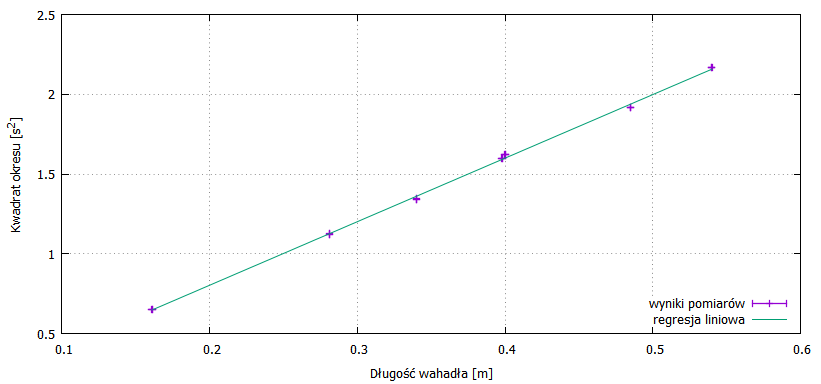
\includegraphics[width=\paperwidth - 50pt]{kwadrat.png}}
	\caption{Wykres zależności kwadratu okresu od długości wahadła}
\end{figure}

 \section{Wnioski}
 
 W powyższym ćwiczeniu dokonano prezentacji pomiaru jednokrotnego, pomiarów wielokrotnych. Wyniki zostały opracowane w oparciu o teorię niepewności pomiarów, której podstawowe zasady przedstawiono w sprawozdaniu. 

	Patrząc na podsumowanie wyników w tabeli \ref{tab} można zobaczyć, że wszystkim grupom udało się wyznaczyć przyspieszenie ziemskie zgodne z wartością tabelaryczną. Trzeci pomiar posiada bardzo dużą niepewność $u(g)$ wynika to najprawdopodobniej z tego, że zmierzony okres jest bardzo krótki, ponieważ długość nici również była  mała. Im krótsza nić tym wahadła szybciej drga i trudniej zmierzyć dokładnie okres.

	Żaden pomiar nie jest idealnie dokładny, wszystkie są obarczone niepewnością pomiaru wynikającą z niedokładności przyrządu pomiarowego, przypadkowości działania ludzkich zmysłów.
	Osobnym problemem jest tzw. błąd gruby. Takie drastyczne różnice między otrzymaną a spodziewaną wartością sugerują popełnienie błędu podczas doświadczenia (błędne obliczenia, pomyłka przy odczytywaniu i zapisie wyników itp.).
\end{document}